% !TeX program = xelatex
%==============================================================
%  Python金融数据分析 · 第8章 数学工具
%  基于《Python金融大数据分析（第2版）》第11章内容改编
%  授课对象：本科金融系学生（已学完第2-7章）
%  编译：xelatex chapter8.tex（编译两遍）
%==============================================================
\documentclass[9pt]{ctexbeamer}

%%%%-----导入宏包-----%%%%
\usepackage{style/shubeamer}   % SHU 主题（配色、帧标题、页脚、Python代码样式）
\usepackage{amsmath,amsfonts,amssymb,bm}
\usepackage{graphicx,hyperref,url}
\usepackage{subcaption}
\usepackage{booktabs}
\usepackage[super,square]{natbib}
\usepackage{wrapfig}          % 文字绕排
\usepackage{calligra}         % 结尾页花体字

%%%%-----设置字体-----%%%%
\setmainfont{CMU Serif}
\setsansfont{CMU Sans Serif}

%%%%-----常用自定义颜色（正文可直接使用）-----%%%%
\definecolor{nvidia}{RGB}{102,156,28}
\definecolor{red}{RGB}{184,13,73}
\definecolor{orange}{RGB}{242,151,36}
\definecolor{darkteal}{RGB}{43,106,108}
\definecolor{darkblue}{RGB}{4,37,58}

%%%%-----每节开始时自动显示当前节目录-----%%%%
\AtBeginSection[]
{
	\begin{frame}<beamer>
		\frametitle{\textbf{目录}}
		\textbf{\tableofcontents[currentsection]}
	\end{frame}
}

%%%%-----设定图片存放路径-----%%%%
\graphicspath{{figures/}}

%%%%-----首页信息设置-----%%%%
\AtBeginDocument{%
	%%%%----短标题[显示在页脚]{封面标题}
	\title[Python金融数据分析 · 第8章]{\fontsize{16pt}{22pt}\selectfont {Python金融数据分析}}
	%%%%----副标题（本章主题）
	\subtitle{\fontsize{9pt}{14pt}\selectfont \textit{第8章\quad 数学工具}}
	%%%%----个人信息
	\author[王伟冠]{%
		\begin{tabular}{ll}%
			主讲人： & 王伟冠\tabularnewline%
			院\quad 系： & 经济学院金融系\tabularnewline
		\end{tabular}
	}
	%%%%----机构信息
	\institute[SHU]{上海大学}
	%%%%----日期信息
	\date[\today]{\today}}

%%%%-----数学宏（向量、矩阵、算子等，见 style/macros.tex）-----%%%%
\input{style/macros.tex}


\begin{document}

%% 封面
\begin{frame}
	\titlepage
\end{frame}

%% 目录页
\section*{目录}
\begin{frame}
	\frametitle{\textbf{目录}}
	\textbf{\tableofcontents}
\end{frame}


%==============================================================
\section{金融为什么需要数学工具}
%==============================================================

\begin{frame}{本章学习目标}
	\begin{itemize}
		\item 会用\textbf{回归}（\texttt{np.polyfit}）与\textbf{插值}（样条）逼近函数与数据
		\item 会用 \texttt{scipy.optimize} 做全局搜索、局部优化与\alert{带约束}优化
		\item 理解数值积分与蒙特卡洛积分，知道它们与期权定价的关系
		\item 初步掌握 SymPy 符号计算：解方程、求导、积分
	\end{itemize}
	\begin{block}{四大工具与金融应用}
		\begin{tabular}{ll}
			逼近（回归/插值） & 收益率曲线补全、美式期权估值 \\
			凸优化 & 模型校准、投资组合选择 \\
			积分 & 衍生品定价（期望收益的折现） \\
			符号计算 & 推导解析公式（如希腊字母） \\
		\end{tabular}
	\end{block}
\end{frame}

\begin{frame}{本章的示例函数}
	\begin{itemize}
		\item 教材用一个"正弦+线性"函数贯穿全章：
	\end{itemize}
	\begin{equation*}
		f(x) = \sin(x) + 0.5\,x
	\end{equation*}
	\begin{itemize}
		\item 它既有弯曲部分（考验拟合能力）又有趋势项，很适合演示逼近方法。
		\item 第6章我们用 \texttt{np.polyfit} 估计过 beta——那就是回归的金融应用；
			本章把它推广为\alert{通用的函数逼近工具}。
	\end{itemize}
	\begin{alertblock}{零基础提醒}
		数学符号不必害怕：本章重点是"会调用、会读图、会解释"，推导细节留给专门课程。
	\end{alertblock}
\end{frame}


%==============================================================
\section{函数逼近：回归}
%==============================================================

\begin{frame}[fragile]{多项式回归：一行拟合}
	\begin{lstlisting}
import numpy as np

def f(x):
    return np.sin(x) + 0.5 * x

x = np.linspace(-2 * np.pi, 2 * np.pi, 50)
reg = np.polyfit(x, f(x), deg=7)   # 7次多项式拟合
ry  = np.polyval(reg, x)           # 用拟合结果求值
np.mean((f(x) - ry) ** 2)          # 均方误差 MSE ≈ 0.0018
\end{lstlisting}
	\begin{itemize}
		\item \texttt{np.polyfit(x, y, deg)}：找一条 \texttt{deg} 次多项式，
			使它与数据点的误差平方和最小（最小二乘）。
		\item \texttt{np.polyval(reg, x)}：把拟合系数代入求值。
		\item MSE 越小拟合越好：1次 $\approx 0.42$，5次 $\approx 0.054$，7次 $\approx 0.0018$。
	\end{itemize}
\end{frame}

\begin{frame}{次数越高越好吗？}
	\begin{figure}
		\centering
		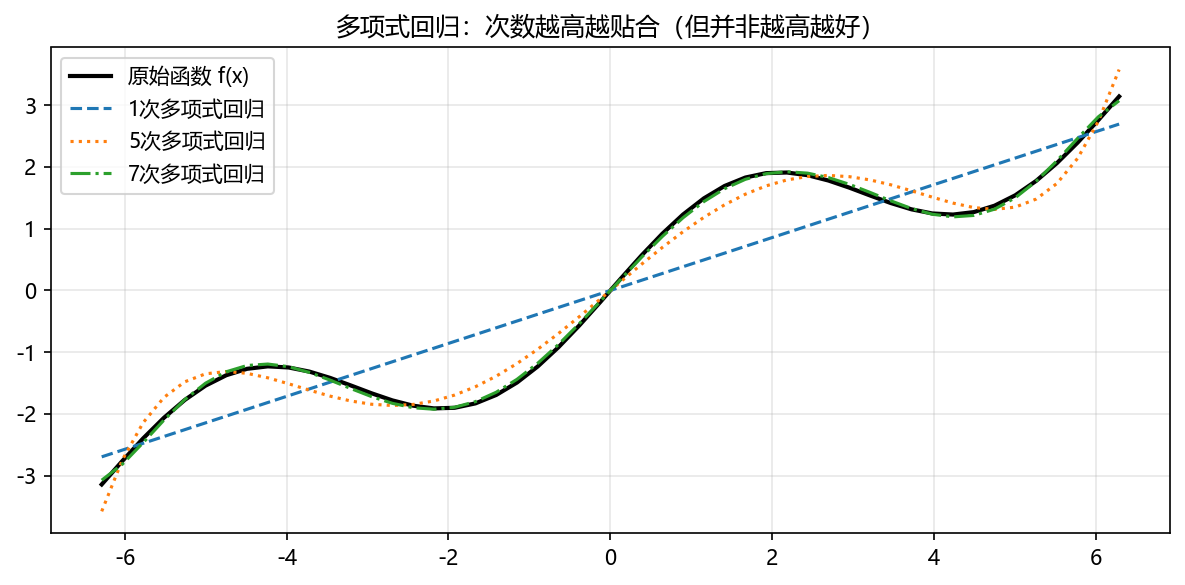
\includegraphics[width=0.85\textwidth]{mt_regression}
		\caption{1次（直线）完全忽略波动；7次几乎完美贴合}
	\end{figure}
\end{frame}

\begin{frame}{回归的两个优点}
	\begin{itemize}
		\item \textbf{抗噪声}：数据带噪声时，回归曲线反而比数据点更接近真实函数
			——它在"平均掉"噪声。
		\item \textbf{不要求排序}：数据点顺序打乱也不影响结果。
	\end{itemize}
	\begin{alertblock}{过拟合警告}
		多项式次数过高时，曲线会穿过每个噪声点、在点之间剧烈震荡——
		对样本"背得滚瓜烂熟"，对新数据一塌糊涂。
		\alert{次数选择要配合样本外检验}（后面的机器学习思想）。
	\end{alertblock}
\end{frame}


%==============================================================
\section{函数逼近：插值}
%==============================================================

\begin{frame}[fragile]{样条插值：平滑地穿过每个点}
	\begin{lstlisting}
import scipy.interpolate as spi

xa = np.linspace(-2 * np.pi, 2 * np.pi, 12)  # 12个观测点
ya = f(xa)
ipo = spi.splrep(xa, ya, k=3)    # 构造三次样条
xs = np.linspace(-2 * np.pi, 2 * np.pi, 200)
iy = spi.splev(xs, ipo)          # 在更密的网格上求值
\end{lstlisting}
	\begin{itemize}
		\item \texttt{splrep}（构造）+ \texttt{splev}（求值），与
			\texttt{polyfit}+\texttt{polyval} 的分工一模一样。
		\item \texttt{k=3}：三次样条——分段三次多项式，连接处平滑可导。
	\end{itemize}
\end{frame}

\begin{frame}{插值的效果}
	\begin{figure}
		\centering
		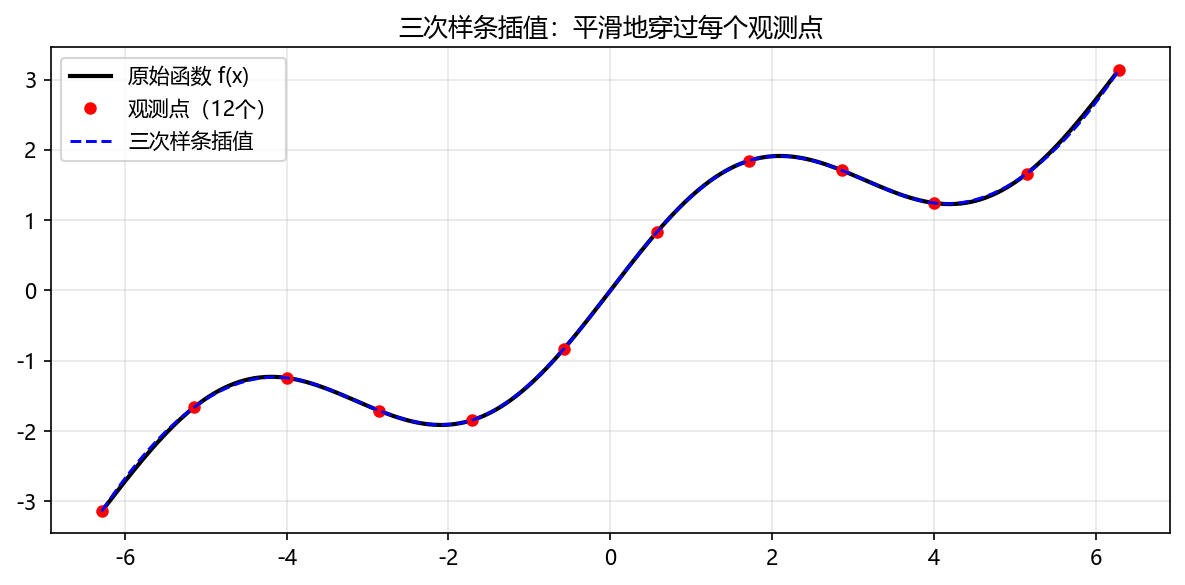
\includegraphics[width=0.85\textwidth]{mt_interp}
		\caption{只用12个点，三次样条就能平滑还原整条曲线}
	\end{figure}
\end{frame}

\begin{frame}[fragile]{金融应用：收益率曲线插值}
	\begin{itemize}
		\item 市场上只有整期限的国债利率：1年、3年、5年、10年\ldots
		\item 定价需要 7.5 年的利率怎么办？——\alert{插值}。
	\end{itemize}
	\begin{lstlisting}
import pandas as pd
maturity = [1, 3, 5, 10]              # 已知期限（年）
rate     = [1.5, 2.1, 2.6, 3.2]       # 对应利率（%）
ipo = spi.splrep(maturity, rate, k=3)
spi.splev(7.5, ipo).round(3)          # 7.5年期利率 ≈ 3.04%
\end{lstlisting}
	\begin{alertblock}{插值的限制}
		要求数据\textbf{有序且无噪声}，高维问题不适用——这正是回归的主场。
	\end{alertblock}
\end{frame}


%==============================================================
\section{优化：寻找最优解}
%==============================================================

\begin{frame}{优化问题长什么样}
	\begin{itemize}
		\item 目标函数有多个"坑"（局部极小值），全局最小值藏在其中：
	\end{itemize}
	\begin{figure}
		\centering
		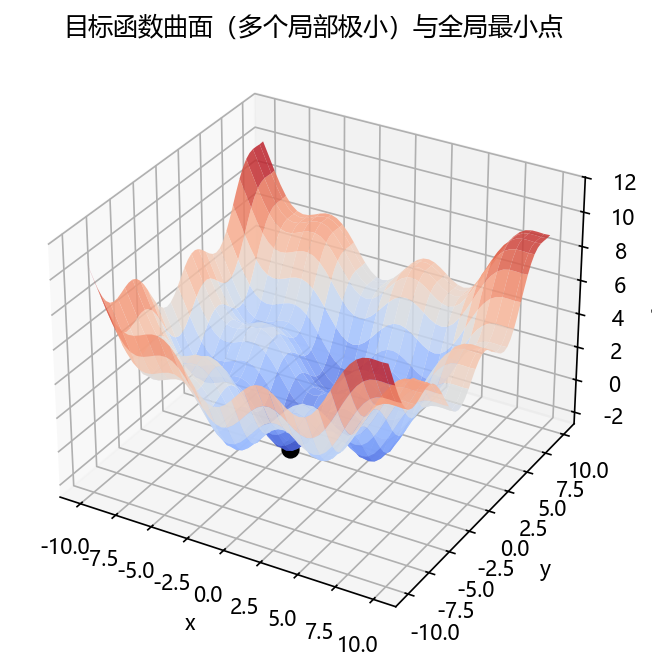
\includegraphics[width=0.62\textwidth]{mt_optim}
		\caption{$f(x,y)=\sin x + 0.05x^2 + \sin y + 0.05y^2$，黑点为全局最小}
	\end{figure}
\end{frame}

\begin{frame}[fragile]{两步走：全局粗搜 + 局部精修}
	\begin{lstlisting}
import scipy.optimize as sco

def fm(p):
    x, y = p
    return np.sin(x) + 0.05 * x ** 2 \
         + np.sin(y) + 0.05 * y ** 2

# 1. 全局：网格上逐点尝试（暴力但可靠）
opt1 = sco.brute(fm, ((-10, 10.1, 0.1), (-10, 10.1, 0.1)),
                 finish=None)          # 找到约 (-1.4, -1.4)
# 2. 局部：从粗搜结果出发精细下降
opt2 = sco.fmin(fm, opt1, xtol=0.001, ftol=0.001, disp=False)
opt2.round(4)    # [-1.4274, -1.4279]，f = -1.7757
\end{lstlisting}
\end{frame}

\begin{frame}{为什么必须先全局后局部？}
	\begin{itemize}
		\item 局部算法（\texttt{fmin}）像"闭眼下山"：从哪出发，就掉进哪个坑。
		\item 从 $(2, 2)$ 出发只能得到 $f \approx 0.02$ 的"局部最优"，
			错过真正的全局最小 $-1.78$。
		\item \texttt{brute} 先在网格上扫一遍，锁定最深的坑，再交给 \texttt{fmin} 精修。
	\end{itemize}
	\begin{alertblock}{金融中的教训}
		模型校准（如用市场报价反推期权模型参数）是典型的优化问题；
		不加全局搜索，可能校准到一个"局部最优"的错误参数组合。
	\end{alertblock}
\end{frame}

\begin{frame}[fragile]{带约束优化：投资组合选择}
	\begin{itemize}
		\item 预算 100 元买两种证券（单价均 10 元）；一年后状态 u/d 等概率，
			收益向量分别为 $(15, 5)$ 与 $(5, 12)$；效用 $u(w)=\sqrt{w}$。
			求最大化期望效用的购买数量。
	\end{itemize}
	\begin{lstlisting}
import math
def eu(p):      # 最小化"负效用" = 最大化效用
    s, b = p
    return -(0.5 * math.sqrt(s * 15 + b * 5)
           + 0.5 * math.sqrt(s * 5 + b * 12))
cons = [{"type": "ineq", "fun":
         lambda p: 100 - p[0] * 10 - p[1] * 10}]  # 预算约束
res = sco.minimize(eu, (5, 5), method="SLSQP",
                   bounds=((0, 10), (0, 10)),
                   constraints=cons)
res.x.round(2)   # [8.03, 1.97]：花光全部预算
\end{lstlisting}
\end{frame}


%==============================================================
\section{积分：从面积到期权价格}
%==============================================================

\begin{frame}{积分 = 曲线下面积}
	\begin{figure}
		\centering
		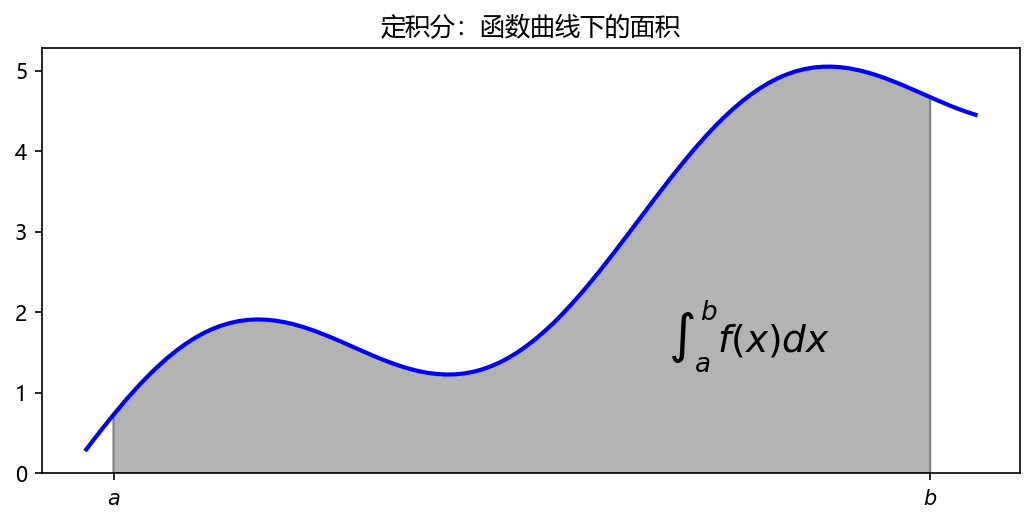
\includegraphics[width=0.7\textwidth]{mt_integral}
		\caption{$\int_{0.5}^{9.5} f(x)\,dx$：衍生品定价的数学本质就是这类计算}
	\end{figure}
\end{frame}

\begin{frame}[fragile]{数值积分：sci.quad}
	\begin{lstlisting}
import scipy.integrate as sci

a, b = 0.5, 9.5
sci.quad(f, a, b)[0]      # 24.37475...（自适应求积，最常用）
\end{lstlisting}
	\begin{itemize}
		\item \texttt{quad} 返回 (结果, 误差估计)，通常取第一个元素。
		\item 数据点形式则用 \texttt{sci.trapz}（梯形法则）。
		\item \textbf{金融意义}：期权在风险中性测度下的价值
			$=$ 期望折现收益；连续情形下，期望就是一个积分。
	\end{itemize}
\end{frame}

\begin{frame}[fragile]{蒙特卡洛积分：用随机数算面积}
	\begin{lstlisting}
rng = np.random.default_rng(1000)
N = 500000
x = rng.random(N) * (b - a) + a    # 区间内均匀撒点
np.mean(f(x)) * (b - a)            # 平均函数值 × 区间长度
# 结果 ≈ 24.36，与 quad 基本一致
\end{lstlisting}
	\begin{itemize}
		\item 原理：$\int_a^b f(x)dx = (b-a)\cdot E[f(x)]$，用样本均值逼近期望。
		\item 样本越多越准，但\alert{收敛不单调}，误差按 $1/\sqrt{N}$ 下降。
	\end{itemize}
	\begin{block}{为什么金融偏爱蒙特卡洛？}
		高维（多资产、多期）积分数值方法会"维度爆炸"，蒙特卡洛的收敛速度却与维度无关——
		它是复杂衍生品定价的主力工具（下下章的主题）。
	\end{block}
\end{frame}

\begin{frame}{蒙特卡洛的收敛过程}
	\begin{figure}
		\centering
		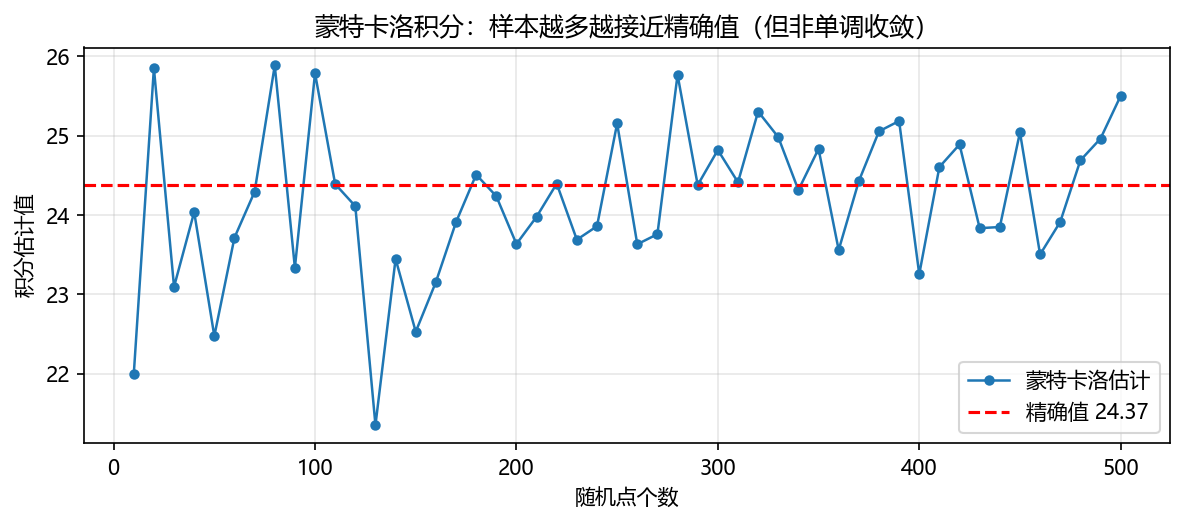
\includegraphics[width=0.85\textwidth]{mt_mc}
		\caption{估计值围绕精确值（红色虚线）震荡收窄}
	\end{figure}
\end{frame}


%==============================================================
\section{符号计算：SymPy}
%==============================================================

\begin{frame}[fragile]{符号对象：让 x 保持为 x}
	\begin{lstlisting}
import sympy as sy

x = sy.Symbol("x")        # x 是符号，不是数字
f = sy.sin(x) + 0.5 * x   # 符号表达式
sy.solve(x ** 2 - 1, x)   # 解方程：[-1, 1]
sy.simplify((x ** 2 - 1) / (x - 1))   # 化简：x + 1
\end{lstlisting}
	\begin{itemize}
		\item NumPy 算的是"数"，SymPy 算的是"式子"。
		\item 在 Notebook 中，SymPy 表达式会以漂亮的数学公式显示。
	\end{itemize}
\end{frame}

\begin{frame}[fragile]{符号微积分}
	\begin{lstlisting}
sy.diff(f, x)                  # 求导：cos(x) + 0.5
sy.integrate(f, x)             # 不定积分：0.25x^2 - cos(x)
sy.integrate(f, (x, 0.5, 9.5)).evalf()   # 定积分：24.3748
\end{lstlisting}
	\begin{itemize}
		\item 与数值积分 \texttt{quad} 的结果完全一致——互相验证的好例子。
		\item 金融应用：期权价格对参数的导数（Delta、Gamma 等"希腊字母"）
			可用符号求导得到解析式。
	\end{itemize}
	\begin{alertblock}{数值 vs 符号}
		要"精确公式"用 SymPy；要"大规模快速计算"用 NumPy/SciPy。两者互补。
	\end{alertblock}
\end{frame}


%==============================================================
\section{小结与练习}
%==============================================================

\begin{frame}{本章小结}
	\begin{itemize}
		\item \textbf{回归}：\texttt{polyfit/polyval}，抗噪声、不要求排序；
			警惕过拟合。
		\item \textbf{插值}：\texttt{splrep/splev}，有序无噪声数据的平滑还原；
			典型应用是收益率曲线。
		\item \textbf{优化}：\texttt{brute}（全局粗搜）$\to$ \texttt{fmin}（局部精修）；
			带约束用 \texttt{minimize + constraints}。
		\item \textbf{积分}：\texttt{quad} 精确快速；蒙特卡洛
			$\bar{f}\times(b-a)$ 通吃高维问题。
		\item \textbf{符号}：SymPy 解方程、求导、积分，推导解析公式。
	\end{itemize}
\end{frame}

\begin{frame}{课后任务与下章预告}
	\begin{block}{课后任务}
		\begin{enumerate}
			\item 对 $g(x)=\cos(x)+0.2x$ 分别做 3 次与 9 次多项式回归，
				比较 MSE 并绘图。
			\item 给定期限 $[1,2,5,10]$ 年、利率 $[1.6, 1.9, 2.5, 3.1]$，
				用三次样条插值估计 3.5 年期利率。
			\item 选做：把蒙特卡洛积分的样本数从 $10^3$ 增加到 $10^6$，
				记录误差变化，验证 $1/\sqrt{N}$ 规律。
		\end{enumerate}
	\end{block}
	\begin{exampleblock}{下章预告}
		数学工具让代码表达力倍增，但循环写多了会变慢。下一章讲 \textbf{性能}：
		为什么向量化比循环快，以及如何科学地计时。
	\end{exampleblock}
	\begin{center}
		\vspace{0.5em}
		本章内容改编自教材第11章\citep{hilpisch2018python}。
	\end{center}
\end{frame}


%==============================================================
%  附录：参考文献 + 结尾页
%==============================================================
\appendix

\begin{frame}[allowframebreaks]{参考文献}
	\bibliographystyle{style/gbt7714-2005}
	\bibliography{reference.bib}
\end{frame}

\begin{frame}
	\begin{center}
		{\Huge\calligra Thanks for your attention!}
		\vspace{1cm}

		{\Huge Q \& A}
	\end{center}
\end{frame}

\end{document}
